\subsection{2D-Tetris Environment}
\subsection{Two-Dimensional Tetris Environment}

\paragraph{Code base.}
Our environment is a thin wrapper around the public \textsc{Tetris-deep-Q-learning-pytorch}\footnote{\url{https://github.com/vietnh1009/Tetris-deep-Q-learning-pytorch}} implementation, which we forked and modularised to decouple game logic from agent code.  The original author exposes a \texttt{Tetris} class that maintains game state, provides a vectorised description of successor states, and computes shaped rewards.  We retain these core routines, but refactor rendering and seeding utilities for reproducibility and batch simulation.

\paragraph{Board geometry and pieces.}
The playfield is a fixed $10 \times 20$ matrix of integers.  Zero denotes empty cells, while positive integers index a global colour table for display.  The canonical tetromino set is represented as binary masks stored in \texttt{Tetris.pieces} at initial orientation.  A \texttt{bag} sampler shuffles these indices and draws without replacement, replicating modern Tetris randomness and eliminating long droughts.  Upon spawn, each piece is horizontally centred at the top row.

\paragraph{Action space.}
An action is a tuple $(x,r)$ where $x\in{0,\dots,W-1}$ is the column of the leftmost block after placement and $r\in{0,1,2,3}$ is the number of clockwise $90^{\circ}$ rotations.  Because rotational symmetries vary by shape, \texttt{get\_next\_states} rules out redundant $r$ values (for example, the square has a single orientation, whereas the line has two).  For the current piece, the method enumerates all legal $(x,r)$, simulates a hard drop until collision, and caches the resulting four-dimensional feature vector described below.

\paragraph{State representation.}
Each post-action board is compressed into

\[
s=\bigl[\ell,\;h,\;b,\;H\bigr]\in\mathbb{R}^4 ,
\]

where $\ell$ is the number of rows cleared by the action, $h$ is the total count of holes, $b$ is aggregate bumpiness, and $H$ is the column-height sum.  The helper \texttt{get\_state\_properties} computes these statistics in $\mathcal{O}(HW)$ time per candidate state.  This low-dimensional summary yields a smaller yet informative input for value-based agents while preserving differentiability with respect to game difficulty.

\paragraph{Transition dynamics and reward.}
The environment's \texttt{step} routine applies $(x,r)$, executes a deterministic fall, stores the piece, and awards

\[
r_t = 1 + W\cdot \ell_t^{\,2}\]

mirroring the quadratic line-clear bonus in classic Tetris.  A penalty of $-2$ is applied on terminal states to discourage early top-outs.  Episodes terminate when the spawn location is occluded.

\paragraph{Extending to pentominoes.}
To probe generalisation, we augment the piece library with the twelve pentominoes each encoded as a five-cell binary mask at minimal bounding box resolution (Figure \ref{fig:pentominoes}). The board size and physics remain unchanged, but the action space expands because many pentominoes span four unique rotations. The four-feature state abstraction and reward equation are reused verbatim to ensure comparability.


\paragraph{Reproducibility notes.}
All experiments fix the random seed before environment construction, log episode trajectories, and use deterministic GPU kernels when available.  The full source, including pentomino shape definitions and unit tests, is released alongside the code repository.

\begin{wrapfigure}{r}{0.45\textwidth}
    \centering
    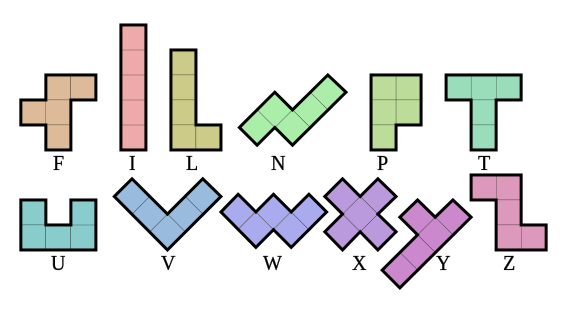
\includegraphics[width=0.45\textwidth]{media/pentomino.png}
    \caption{The twelve pentominoes used in our experiments.}
    \label{fig:pentominoes}
\end{wrapfigure}


\subsection{2D-Tetris Training}

\subsection{Training the Deep Q Network agent}

We adopt a Deep Q Network agent (DQN) with value-based approach in which every legal \texttt{(rotation,,column)} pair is scored by a three-layer multilayer perceptron.  The network processes the four-element state through two hidden layers of 64 rectified linear units before emitting a single action value.  All parameters are initialised with Xavier uniform weights and zero biases.

\paragraph{Experience collection and replay.}
During training the agent interacts with the simulator in an episodic loop in which actions are selected via an epsilon-greedy policy. Epsilon is annealed linearly from one to five times ten to the minus four over three hundred thousand training steps, after which it is held constant.  Every transition tuple is stored in a FIFO replay buffer that holds 30000 entries.  Once the buffer contains at least ten per cent of its capacity, updates commence: a random batch of up to five hundred and twelve samples is drawn, the one-step bootstrap target is computed, and the mean-squared error loss is minimised with Adam at a learning rate of one times ten to the minus four.

\paragraph{Baseline tetromino configuration.}
For the classic seven-piece game we train for three hundred thousand epochs.  All other hyperparameters follow the default values listed above.  Training statistics such as episodic score, pieces placed, cleared lines, and instantaneous loss are logged to TensorBoard each epoch, and human-readable averages are printed every two hundred epochs to monitor stability.

\paragraph{Pentomino extension.}
Introducing the five-block shapes greatly enlarges the action space and amplifies the prevalence of holes and surface roughness.  To compensate we expand the network to a three-layer MLP with 256 hidden units per layer. We also lengthened optimisation to five hundred thousand epochs, allowing the moving epsilon schedule to reach its exploitation regime. Learning rate was tuned to $10^{-4}$, and the batch size was increased to 1024 to accommodate the larger state space. Reward shaping is left intact to keep the comparative analysis between tetromino and pentomino runs straightforward.

\paragraph{Evaluation protocol.}
After training, the checkpoint with the highest validation score is loaded as the agent plays with pure exploitation, selecting the greedy action at every step and recording cumulative score, pieces placed, and cleared lines until game over. The same script can optionally dump an annotated video for qualitative inspection.